\chapter{Insertion Sort}

\section{Introduzione}
Iniziamo la trattazione parlando dell'insertion sort: questo è uno degli algoritmi di sorting più lenti, poichè (partendo dal secondo elemento dell'array) confronta ogni elemento $i$-esimo con i suoi precedenti da $0$ a $i-1$ e, se ne trova uno maggiore, lo scambia con esso. 

Intuitivamente è molto semplice, ma come spesso accade, più è semplice l'implementazione e più il tempo di esecuzione risulta elevato, poiché l'algoritmo non è efficiente. Come vantaggio, però, abbiamo l'ordinamento sul posto, cioé la necessità di un buffer costante per ordinare (in questo caso un buffer di dimensione uno, cioé una variabile).

\section{Tempo di esecuzione}

%\begin{algorithm}
%\begin{algorithmic}[1]
%	\Procedure{InsertionSort}{$A$}
%	\For{$j \gets 2 $ to $length[A]$}\label{ins:for}
%	\State $key \gets A[j]$
%	\State $i \gets j - 1$
%	\While{$i>0$ and $ key < A[i]$}\Comment{Tecnica del cortocircuito}\label{ins:while}
%	\State $A[i+1] \gets A[i]$
%	\State $i \gets i-1$
%	\EndWhile
%	\State $A[i+1] \gets key$
%	\EndFor
%	\EndProcedure
%\end{algorithmic}
%\end{algorithm}
%
%Valutando lo pseudocodice, possiamo notare come il ciclo for a riga \ref{ins:for} viene eseguito $n-1$ volte (dove con $n$ indicheremo - anche nel seguito - la lunghezza del vettore da ordinare, cioé $length[A]$), mentre il ciclo while a riga \ref{ins:while} può eseguire almeno 0 volte (nel caso in cui il vettore sia già ordinato in senso crescente, e quindi ogni confronto $key < A[i]$ darà sempre $false$) o al più $n-1$ volte (nel caso stavolta che il vettore sia ordinato in senso decrescente).
%
%Risulta evidente che il tempo migliore è $T(n) = \Theta(n)$, mentre il tempo peggiore è $T(n) = \Theta(n^{2})$. Nel caso medio, com'è ovvio, $T(n)$ è compreso fra $\Theta(n)$ e $\Theta(n^2)$; per riassumere la scrittura, diremo che $T(n) = O(n^{2})$, cioé che il suo tempo massimo può coincidere con una funzione quadratica.
%
%Questo risultato, del tutto teorico, è anche corroborato dal risultato sperimentale ottenuto generando al calcolatore diversi array di dimensioni elevate in maniera randomica, ordinando tali array con insertion sort, misurando i tempi ottenuti e plottando il tutto su \mbox{Matlab}.

\begin{figure}[h]
	\centering
	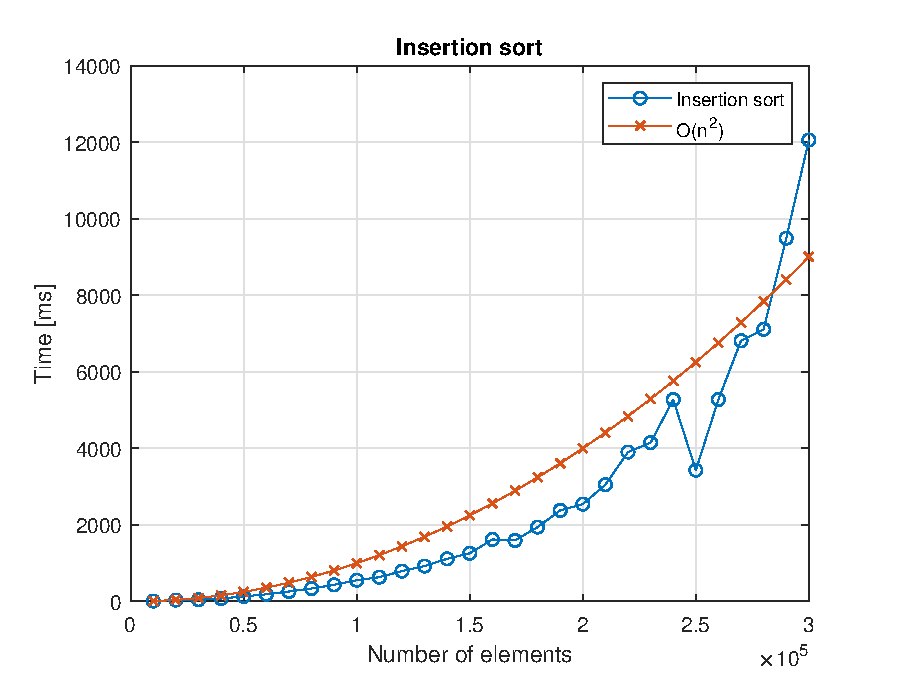
\includegraphics{./insertion/graph.eps}
	\captionAlgorithm{Insertion Sort}
	\label{ins:fig}
\end{figure}

Come abbiamo studiato, l'Insertion Sort ha un tempo di esecuzione $T(n) = \Omega(n) = O(n^2)$, quindi compreso fra un andamento lineare e uno quadratico.

Come possiamo effettivamente notare dal grafico \ref{ins:fig}, notiamo chiaramente che il tempo di esecuzione di Insertion Sort cresce quasi quadraticamente con l'aumentare del numero di elementi da ordinare.
Per plottare $O(n^{2})$ abbiamo usato la funzione $f(n) = an^{2}$, con $a=10^{-7}$.

Come possiamo notare, aumentando il numero degli elementi da ordinare (verso i $3*10^{5}$ elementi), aumenta di molto il tempo di esecuzione rispetto all'andamento di $f(n)$: cambiando il fattore moltiplicativo $a$, ed eventualmente aggiungendo un termine lineare, possiamo tener conto di questi spike temporali e rimanere al di sopra della $T(n)$ misurata.